\begin{comment}
	\pagebreak
\end{comment}

\section{Reinforcement Learning}

\textbf{Return:} $G_t = \sum^\infty y^k R_{t+k+1}$\\
\textbf{Value:} $v_\pi(s) ) \E_\pi[G_t | S_t = s] = \sum_a \pi(a|s) \sum_{s'} \sum_r p(s', r| s,a)[r + \gamma \E_\pi[G_{t+1} | S_{t+1} = S']]$\\
\begin{comment}
	The second term is just the weighted sum of rewards given the current state and action.
	The full thing is just also weighted by the current state and action taken.\\
\end{comment}

\textbf{Q-Func:} $q_\pi(s, a) = \E_\pi[G_t | S_t = s, A_t = a]$\\
\begin{comment}
	Helps when transition function is not given, as it models the value after a certain action, instead of considering all actions.\\
\end{comment}

\textbf{Bellman equation:} $v_\pi(s) = \sum_a \pi(a|s) \sum_{s', r} p(s', r| s,a)[r + \gamma v_\pi(s')]$\\
\begin{comment}
	What it tells us is that we can decompose the state-value function into immediate reward plus the discounted value of the successor state.\\
\end{comment}

\textbf{Greedy value policy:} $\pi'(s) = \argmax(r(s,a) + \gamma V_\pi(p(s,a)))$\\
\begin{comment}
	\Note{One can show that this greedy policy is always at least as good as any other policy}\\
\end{comment}

\textbf{DP:}\\
\begin{comment}
	Pros:
	\begin{itemize}
	\item Exact
	\item Guaranteed to converge in finite time
	\item Value iterarion more efficient than policy iteration	
	\end{itemize}
	
	Cons:
	\begin{itemize}
	\item Need to know transition probability matrix
	\item Need to iterate over the whole state space
	\item Memory proportional to state space	
	\end{itemize}
\end{comment}

\textbf{TD learning:} $\Delta V(s) = r(s,a) + \gamma V(s') - V(s)$, $V(s) \leftarrow V(s) + \alpha \Delta V(s)$\\
\begin{comment}
	Only update value function of visited states.\\
	Random policy would lead to bias in close states.
	Greedy policy would find rewards quickly, but gets stuck quickly.
	$\epsilon$-Greedy, use greedy, but with a certain probability choose random.\\
	
	Pros:
	\begin{itemize}
	\item Less variance than MC
	\item Sample efficient (no need to update all transitions)
	\item No need to know transition probability	
	\end{itemize}
	
	Cons:
	\begin{itemize}
	\item Biased due to bootstrapping
	\item Exploration/ Exploitaition?
	\end{itemize}
	
\end{comment}

\textbf{SARSA:} $\Delta Q(S,A) = R + \gamma Q(S', A') - Q(S, A)$, $Q(S, A) \leftarrow Q(S, A) + \alpha \Delta Q(S, A)$\\
\begin{comment}
	On-policy method, because we are using the current policy to get the rewards from Q\\
\end{comment}

\textbf{Q-Learning:} $\Delta Q(S,A) = R_{t+1} + \gamma \max_a[Q(S', a)] - Q(S, A)$, $Q(S,A) \leftarrow Q(S, A) + \alpha \Delta Q(S, A)$\\
\begin{comment}
	Off-policy, because the policy we use to update the Q function is different from the policy we use to collect the data\\
\end{comment}

\textbf{Deep Q:} $\cL(\theta) = (R + \gamma \max_{a'}[Q_\theta(S', a')] - Q_\theta(S,A))^2$\\
\begin{comment}
	SGD assumes i.i.d: Use replay buffer in training phase and randomly sample transition from the buffer to update. 
	Since Q-learning is off-policy, we are allowed to use old samples\\
	This is a value based method, we try to optimise the value return, thus indirectly exploiting the problem structure to solve the problem.
	The problem at hand is a regression problem.\\
	
	\begin{Figure}
 		\centering
 		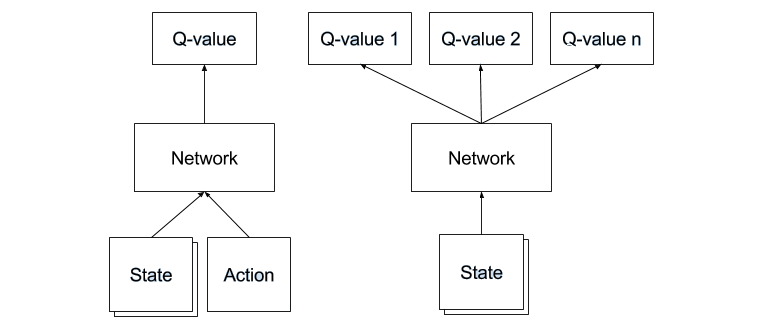
\includegraphics[width=\linewidth]{graphic/rl-deep-q}
 		\captionof{figure}{RL Deep-Q network}
	\end{Figure}
\end{comment}

learn $\pi: S_t \rightarrow A_t$ and $v_\pi: S_t \rightarrow V(S_t)$ as NN\\

\textbf{Policy Gradient:} $\pi(a_t|s_t) = \cN(\mu_t, \sigma_t^2 | s_t)$. $p(\tau) = p(s_1)\prod \pi(a_t|s_t) p(s_{t+1} | a_t, s_t)$\\
\begin{comment}
	\Note{The network is predicting $\mu$ and $\sigma$, which determine the gaussian }\\
	We try to make good trajectories more likely, this is a policy method, as we are optimizing the policy directly.
	Policy methods are used when the action space is really large or continues, we can learn the probabilities for every action directly. 
	It is a classification problem.
	Compared to Q-learning, it is less sample efficient, because we always need to create new samples and can't just reuse the replay buffer.\\
	
	\begin{Figure}
 		\centering
 		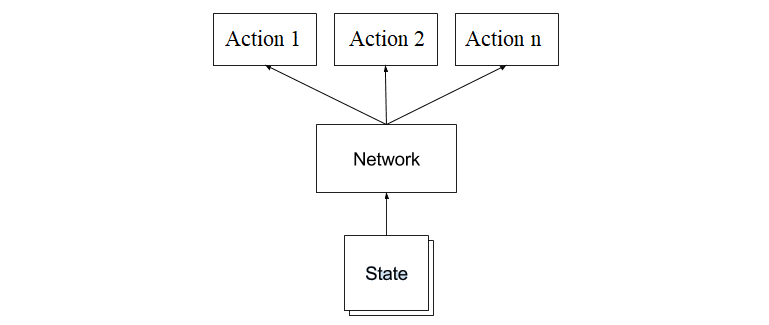
\includegraphics[width=\linewidth]{graphic/rl-policy-network}
 		\captionof{figure}{RL Policy Gradient network}
	\end{Figure}
\end{comment}

\textbf{Update:} $\theta^* = \argmax J(\theta)$, $\theta = \theta + \nabla_\theta J(\theta) = \E_{\tau \sim p(\tau)}[(\sum^T \nabla_\theta \log \pi_\theta(a_t^i | s_t^i))(\sum^T y^t r(s_t^i, a_t^i))]$\\
\begin{comment}
	The first term of the gradient is pointing into the maximum likelihood direction in parameter space, whereas the trajectory reward is scaling this update vector.
	If the reward is high, we want to make it more likely, if the reward is low, we want to make it less likely.\\
\end{comment}

\textbf{Reinforce:} $\nabla_\theta J(\theta) = \frac{1}{N} \sum_i[(\sum^T \nabla_\theta \log \pi_\theta(a_t^i | s_t^i))(\sum^T y^t r(s_t^i, a_t^i) - b(s_t^i))]$\\
\begin{comment}
	Use a baseline to reduce the variance of the discounted rewards\\
\end{comment}

\textbf{Actor-Critic:} $\nabla_\theta J(\theta) = \frac{1}{N} \sum_i \sum^T \nabla_\theta \log \pi_\theta(a_t^i | s_t^i)(r(s_t^i, a_t^i) + \gamma V(s_{t+1}^i) - V(s_t^i))$\\
\begin{comment}
	This is again the temporal difference error\\
\end{comment}





